%# -*- coding:utf-8 -*-
\documentclass[10pt,aspectratio=169,mathserif]{beamer}		
%设置为 Beamer 文档类型,设置字体为 10pt,长宽比为16:9,数学字体为 serif 风格

%%%%-----导入宏包-----%%%%
\usepackage{ccnu}			%导入 CCNU 模板宏包
\usepackage{ctex}			%导入 ctex 宏包,添加中文支持
\usepackage{amsmath,amsfonts,amssymb,bm}   %导入数学公式所需宏包
\usepackage{color}			 %字体颜色支持
\usepackage{graphicx,hyperref,url}
\usepackage{algorithm, algorithmic}
\usepackage{cite}
\usepackage{multirow}
\usepackage{metalogo}	% 非必须
%% 上文引用的包可按实际情况自行增删
%%%%%%%%%%%%%%%%%%	


\beamertemplateballitem		%设置 Beamer 主题
\usecolortheme{dove}
%%%%------------------------%%%%%
\catcode`\。=\active         %或者=13
\newcommand{。}{.}				
%将正文中的“。”号转换为“.”。中文标点国家规范建议科技文献中的句号用圆点替代
%%%%%%%%%%%%%%%%%%%%%

%%%%----首页信息设置----%%%%
\title[课程报告]{生物智能算法}
\subtitle{——群聚算法}			
%%%%----标题设置


\author[Swarm Intelligence]{
  小组成员名字 \\\medskip
  {\small \url{fengliangming@zju.edu.cn}} \\
  {\small \url{http://www.zju.edu.cn/}}}
%%%%----个人信息设置
  
\institute[ZJU]{
  计算机科学与技术学院 \\ 
  浙江大学}
%%%%----机构信息

\date[Apr. 01 2018]{
  2018年04月01日}
%%%%----日期信息
  
\begin{document}

\begin{frame}
\titlepage
\end{frame}				%生成标题页

\section{提纲}
\begin{frame}
\frametitle{提纲}
\tableofcontents
\end{frame}				%生成提纲页

\section{群算法聚介绍}
\begin{frame}
  \frametitle{简介}
	 \begin{enumerate}
	    \item what
	    \item where
	    \item how
	    \item 。。。
	  \end{enumerate}
\end{frame}



\section{蚁群算法}

\begin{frame}
\newcommand{\song}{\setCJKfamilyfont{song}}
\newcommand{\xiaoer}{\fontsize{18pt}{18pt}\selectfont}
	\begin{center}
	{\song\xiaoer\textbf{蚁群算法}}
	\end{center}
\end{frame}


\begin{frame}
	\frametitle{ACO背景}
	蚁群优化算法(Ant Colony Optimizer,ACO)是一种模拟蚁群觅食行为的群聚智能算法,由Marco Dorigo等人在1991年提出。他们根据蚁群通过分泌信息素来交流觅食信息从而能快速的找到目标这一现象,提出了基于信息正反馈原理的蚁群算法。蚁群算法最初用来解决最短路径问题,现在也渐渐应用到了其他领域中。蚁群算法参数较少,设置简单,有很大的改进空间,易于应用到其他组合优化问题中,但同时蚁群算法也有收敛速度慢、易陷入局部最优的缺点。
\end{frame}


\begin{frame}
	\frametitle{ACO生物学模型}
	\begin{columns}
		\column{.4\textwidth}
			\begin{itemize}
				\item{蚂蚁将信息素沉积在地面上,并以概率的方式跟随其他蚂蚁先前留在地面上的信息素。}
			\end{itemize}
			\begin{itemize}
				\item{蚁群利用信息素找到从巢穴到食物源的最短路径。}
			\end{itemize}		
		\column{.6\textwidth}
			\begin{figure}
				\centering
				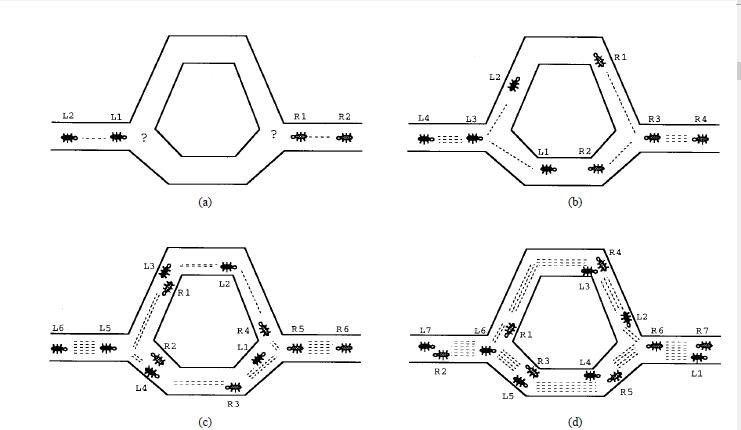
\includegraphics[width=8cm]{pic/ant1.png}
				\caption{蚂蚁觅食}
		\end{figure}
	\end{columns}	
\end{frame}


\begin{frame}
	\frametitle{ACO算法原理-TSP问题定义}
	\begin{columns}
		\column{.5\textwidth}
		\begin{itemize}
			\item{所有城市的集合$C=\left\{ a,b,c…,z \right\}$}
			\item{城市r和s之间的欧几里得距离$d(r,s)$}
			\item{城市r和s之间的信息素$\tau(r,s)$}
		\end{itemize}
		\column{.5\textwidth}
		\begin{figure}[htbp]
			\centering
			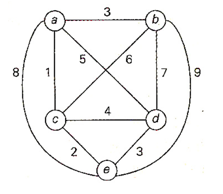
\includegraphics[width=5cm]{pic/ant2.png}
			\caption{TSP问题}
		\end{figure}
	\end{columns}
	TSP问题的目的就是在完全图G中找出距离最短的哈密顿回路,蚁群算法通过概率转移准则、局部更新准则和全局更新准则来达到求解目的。
\end{frame}


\begin{frame}
	\frametitle{ACO算法原理-概率转移准则}
	蚂蚁k在城市r上,选择向下一个城市s移动的概率是:
	\Large{
	$$
	P_k(r,s) =
		\begin{cases}
		\frac{\tau (r,s) \centerdot \eta (r,s)^\beta}{\sum_{u \subset J_{k(r)}} \tau (r,u)\centerdot \eta (r,u)^\beta}  & \text{$,if\quad s \subset J_{k(r)}$ } \\
		0 & \text{$,otherwise$}
		\end{cases}
	$$}
	\normalsize{
	\begin{itemize}
			\item{$J_k(r) = \{ C-tabu_k \}$ 表示蚂蚁下一步可选择的城市}
			\item{$\eta = 1/d$ 启发函数}
			\item{$\beta(\beta>0)$调参数,决定了$\tau$和$\eta$之间的权重}
		\end{itemize}
	}
\end{frame}


\begin{frame}
	\frametitle{ACO算法原理-局部更新准则}
	在构建TSP问题的解的过程中,蚂蚁每访问一条边,就要用局部更新准则去更新边上的信息素。更新原则是:
	\Large{$$\tau(r,s) = (1-\alpha)\centerdot\tau(r,s)+\alpha\centerdot\Delta\tau(r,s)$$}
	\begin{itemize}
			\item{$0<\alpha<1$ }
			\item{$\Delta\tau(r,s) = \gamma\centerdot\max_{z\subset J_{k(s)}}\tau(s,z)$ /
					$\Delta\tau(r,s) = \tau_0$}
		\end{itemize}
\end{frame}


\begin{frame}
	\frametitle{ACO算法原理-全局更新准则}
	全局更新发生所有的蚂蚁都完成了解得构建之后。更新原则是:
	\Large $$\tau(r,s) = (1-\rho)\centerdot\tau(r,s)+\rho\centerdot\Delta\tau(r,s)$$
	$$ where\quad
	\Delta\tau(r,s) =
	\begin{cases}
	(L_{gb}^{-1})  & \text{$,if\quad (r,s) \subset global\quad best\quad tour$ } \\
	0 & \text{$,otherwise$}
	\end{cases}
	$$
	\begin{itemize}
			\item{$0<\rho<1$ \normalsize{挥发系数}}
			\item{$L_{gb}$ \normalsize{当前最短路径的长度}}
		\end{itemize}
\end{frame}


\begin{frame}
	\frametitle{ACO算法原理}
	\begin{algorithm}[H]
	\caption{ACO}\label{wolf_alg}
	\algsetup{linenosize=\tiny} \scriptsize
		\begin{algorithmic}
			\STATE{Initialize}
			\STATE{\textbf{Loop /* at this level each loop is called an iteration */}}
				\STATE{$\qquad$Each ant is positioned on a starting node}
				\STATE{\textbf{$\qquad$Loop /* at this level each loop is called a step */}}
					\STATE{$\qquad\qquad$Each ant applies a state transition rule to incrementally build a solution and a local pheromone updating rule}
				\STATE{$\qquad$\textbf{Until} all ants have build a complete solution}
				\STATE{$\qquad$A global pheromone updating rule is applied}
			\STATE{\textbf{Until} End conditon}
		\end{algorithmic}
	\end{algorithm}
\end{frame}


\begin{frame}
	\frametitle{ACO缺点及改进}
	\begin{columns}
	\column{.5\textwidth}
		\begin{itemize}
		\item {缺点}
			\begin{itemize}
				\item {收敛速度慢}
				\item {易陷入局部最优}
			\end{itemize}
		\item {改进}
			\begin{itemize}
				\item {MMAS(Max Min Ant System)}
				\item {局部搜索算法2-opt(2-Optimization)}
				\item {启发式信息修正}
				\item {蚁群算法与其他仿生算法结合}
			\end{itemize}
		\end{itemize}
	\column{.5\textwidth}
		\begin{figure}[htbp]
			\centering
			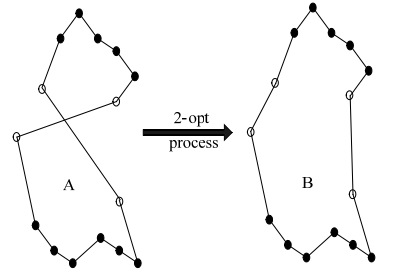
\includegraphics[width=6cm]{pic/ant5.jpg}
			\caption{2-opt搜索}
		\end{figure}
	\end{columns}
\end{frame}


\begin{frame}
	\frametitle{ACO改进-启发式信息修正}
	\begin{itemize}
		\item {启发函数可以在蚂蚁搜索路径的过程中产生一定的影响,因此启发式信息的动态修正是一种有效的改进方法}
		\item {路径期望值:当所有蚂蚁完成一次周游后,将所有的搜索结果按照距离长度递增排序,为$p_1,p_2,…,p_r$,其中r是有效结果的数目,则蚂蚁下次周游时的路径期望值为:$$ P_{Expect}= \sum_{i=1}^{r} (r+1-i)\times p_i/r $$}
		\item {启发函数的调整规则:
		$$
		D_{ij} =
		\begin{cases}
		P_{Expect}-P_{Visited}-d_{ij}  & \text{$if\quad (P_{Expect}-P_{Visited}-d_{ij})>0$ } \\
		0 & \text{$else$}
		\end{cases}
		$$
		$$ \eta_{ij} = \frac{D_{ij}}{\sum D_{is}},\quad s\subset allowed_i$$}
	\end{itemize}
\end{frame}


\begin{frame}
	\frametitle{ACO的其他应用}
	\begin{columns}
	\column{.6\textwidth}
		\begin{itemize}
			\item {车辆路径规划:给定车辆的载重量$Q$,每个客户的需求量$q_i$,车辆数目$m$,要求规划处一条车辆总行程最短的运输方案。}
			\item {图着色优化问题:给定无向连通图$G$和$m$种不同的颜色,用这些颜色给$G$中各顶点着色,且$G$中任意相邻的两个顶点颜色不同,使得$m$最小。}
		\end{itemize}
	\column{.4\textwidth}
		\begin{figure}[htbp]
			\centering
			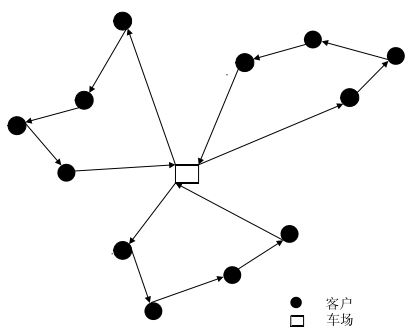
\includegraphics[width=6cm]{pic/ant6.jpg}
			\caption{车辆路径规划}
		\end{figure}
	\end{columns}	
\end{frame}


\begin{frame}
	\frametitle{ACO的其他应用-图着色优化问题}
	\begin{itemize}
		\item {无向图$G=(V,E)$,颜色集$C=\left\{ c_1,c_1,…,c_p \right\}$,用$m$只蚂蚁对其进行遍历着色,每只蚂蚁维持一张着色表$S(n \times p)$
		$$
		S(i,j) =
		\begin{cases}
		0,  & \text{表示不给$v_i$着$c_j$色 } \\
		1, & \text{表示不给$v_i$着$c_j$色}
		\end{cases}
		\qquad \sum_{j=1}^{p}S(i,j)=1
		$$}
		\item {每只蚂蚁维持一个已着色集,记录已经使用过的颜色}		
		\item {所有的蚂蚁共用一张信息素表$\tau (n\times p)$,$\tau (i,j)$表示给$v_i$ 着$c_j$ 色的信息素数量}
		\item {$\Delta_k \tau (i,j)$表示蚂蚁$k$给$v_i$ 着$c_j$ 色时释放的信息素数量}
	\end{itemize}
\end{frame}


\begin{frame}
	\frametitle{ACO的其他应用-图着色优化问题}
	\begin{itemize}
		\item {信息素更新准则:
		$$
		\tau (i,j)= (1-\rho)\centerdot \tau(i,j)+\rho \centerdot \Delta \tau(i,j)
		$$
		$$
		\Delta \tau(i,j) = \sum_{k=1}^{m}\Delta_k \tau(i,j)
		$$
		$$
		\Delta_k \tau(i,j) = Q/Num_c
		$$}
		\item {$Num_c$表示$v_{i-1}$ 着色后使用的总颜色数}
	\end{itemize}
\end{frame}


\begin{frame}
	\frametitle{ACO的其他应用-图着色优化问题}
	概率转移准则:
	\Large{
	$$
	P_k(i,j) =
		\begin{cases}
		\frac{\tau (i,j)^\alpha \centerdot \eta ((i,j)^\beta}{\sum \tau (i,j)^\alpha \centerdot \eta (i,j)^\beta}  & \text{$,if\quad c_j \subset allowed_i^k$ } \\
		0 & \text{$,otherwise$}
		\end{cases}
	$$}
	\normalsize{
	\begin{itemize}
		\item {$allowed_i^k$表示蚂蚁$k$给$v_i$着色时在已着色集中的可行着色集}
		\item {若$allowed_i^k$不为空集,则由转移准则给出$v_i$ 着$c_j$ 色的概率}
		\item {若$allowed_i^k$为空集,则$Num_c= Num_c+1$,并给$v_i$着$c_{Num_c}$色,再把$c_{Num_c}$色放入已着色集中}
	\end{itemize}
	}
\end{frame}

\section{鱼群算法}
\begin{frame}
  \frametitle{fish}
	 \begin{enumerate}
	    \item test
	    \item test
	    \item test
	    \item test
	  \end{enumerate}
\end{frame}

\section{蜂群算法}
\begin{frame}
\newcommand{\song}{\setCJKfamilyfont{song}}
\newcommand{\xiaoer}{\fontsize{18pt}{18pt}\selectfont}
	\begin{center}
	{\song\xiaoer\textbf{人工蜂群算法}}
	\end{center}
\end{frame}

\begin{frame}
  \frametitle{ABC算法背景}
	\qquad 人工蜂群算法(Attificial Bee Colony,ABC)算法是由土耳其学者Karaboga于2005年提出,其基本思想是启发 	 	于蜂	群通过个体分工和信息交流,相互协作完成采蜜任务。与传统的优化方法相比,它的主要优点是不需要了解问    	题的特殊信息,只需要对解进行优劣比较,通过人工蜂群个体的局部寻优行为,最终在群体中使得全局最优值	 	凸现出来,具有较快的收敛速度。
\end{frame}

\begin{frame}
	\frametitle{自然界的蜂群}
	\begin{columns}
	\column{.4\textwidth}
		\section{觅食行为}
		\begin{itemize}
			\item { 3个基本要素}
				\begin{itemize}
					\item { 蜜源Food Source}
					\item { 被雇佣蜂(引领峰)Employed Foragers}
					\item { 未被雇佣蜂Unemployed Foragers}
						\begin{itemize}
							\item { 跟随蜂 }
							\item { 侦查蜂 }
						\end{itemize}
				\end{itemize}
			\item { 2种基本行为}
				\begin{itemize}
					\item {为蜜源招募蜜蜂Recruit}
					\item {放弃蜜源Abandon}
				\end{itemize}
			 \item { 信息交流}
				\begin{itemize}
					\item {舞蹈区:摇摆舞}
				\end{itemize}
		\end{itemize}
	\column{.6\textwidth}
		\begin{itemize}
			\item[ ] 
				\begin{figure}[htbp]
					\centering
					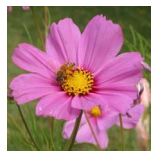
\includegraphics[scale=0.5]{pic/bee1.png}
				\end{figure}
			\item[ ]
				\begin{figure}[htbp]
					\centering
					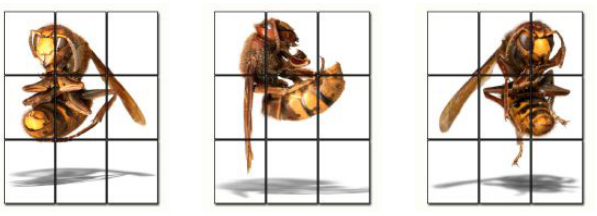
\includegraphics[scale=0.5]{pic/bee2.png}
				\end{figure}
			\item[ ] 
				\begin{figure}[htbp]
					\centering
					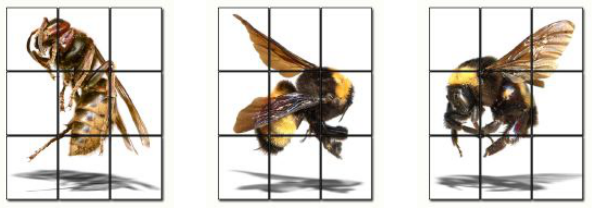
\includegraphics[scale=0.5]{pic/bee3.png}
				\end{figure}
		\end{itemize}
	\end{columns}
\end{frame}


\begin{frame}
	\frametitle{自然界的蜂群}
	\begin{columns}
	\column{.6\textwidth}
		\begin{itemize}
			\item {引领蜂的搜索行为}
				\begin{itemize}
					\item {在舞蹈区进行蜜源信息分享后,发现自己的蜜源质量并不高,放弃蜜源重新变成侦查蜂寻找新蜜源(图中UF线)}
					\item {在舞蹈区跳摇摆舞招募蜜蜂,此时蜂巢里的非雇佣蜂以一定概率跟随引领蜂回到蜜源进行采蜜(图中EF1线)}
					\item {继续在蜜源处采蜜而不进行招募(图中EF2)}
				\end{itemize}
			\item {非雇佣蜂的搜索行为}
				\begin{itemize}
					\item {以侦查蜂的身份,自发搜索蜂巢附近的蜜源(图中S线)}
					\item {在观察完摇摆舞被雇佣成为跟随蜂,开始搜索对应蜜源附近并采蜜(图中R线)}
				\end{itemize}
		\end{itemize}
	\column{.4\textwidth}
		\begin{figure}[htbp]
			\centering
			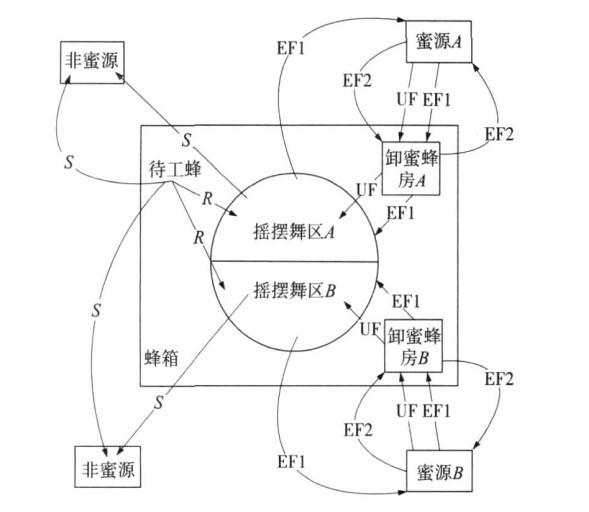
\includegraphics[width=6cm]{pic/bee4.jpg}
		\end{figure}
	\end{columns}
\end{frame}


\begin{frame}
	\frametitle{自然界的蜂群}
	\begin{columns}
	\column{.6\textwidth}
		\begin{itemize}
			\item {角色转换}
				\begin{itemize}
					\item {引领蜂用于维持优良解(记录当前局部最优解)。}
					\item {跟随蜂用于提高收敛速度(搜索局部最优解的附近空间)。}
					\item {侦查蜂用于增强摆脱局部最优的能力(重新全局搜索)。}
				\end{itemize}
		\end{itemize}
	\column{.4\textwidth}
		\begin{figure}[htbp]
			\centering
			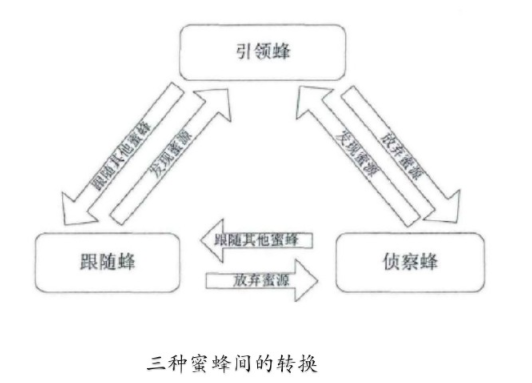
\includegraphics[width=6cm]{pic/bee5.png}
		\end{figure}
	\end{columns}
\end{frame}

\begin{frame}
	\frametitle{ABC算法模型}
	\begin{columns}
	\column{.6\textwidth}
	\qquad 首先初始化种群,派出侦查蜂搜索蜜源,找到蜜源后转换为引领蜂并评估蜜源的质量,所有引领蜂搜索完毕后回到蜂巢,令适应度高的蜜源对应的引领蜂招募跟随蜂,并对蜜源进行邻域搜索,保留较好的解;令适应度低的蜜源对应的引领蜂重新成为侦查蜂搜索新的蜜源,不断循环输出最优解。
	\column{.4\textwidth}
	\begin{table}[]
	\centering
	\caption{采蜜行为与优化问题的映射}
	\label{采蜜行为与优化问题的映射}
	\begin{tabular}{ccll}
	\cline{1-2}
	\multicolumn{1}{|c|}{\textbf{蜂群采蜜行为}} & \multicolumn{1}{c|}{\textbf{优化问题}} &  &  \\ \cline{1-2}
	\multicolumn{1}{|c|}{蜜源位置}            & \multicolumn{1}{c|}{可行解}            &  &  \\ \cline{1-2}
	\multicolumn{1}{|c|}{蜜源质量}            & \multicolumn{1}{c|}{适应度}            &  &  \\ \cline{1-2}
	\multicolumn{1}{|c|}{采蜜速度}            & \multicolumn{1}{c|}{收敛速度}           &  &  \\ \cline{1-2}
	\multicolumn{1}{|c|}{食物源质量最大值}        & \multicolumn{1}{c|}{最优解}            &  &  \\ \cline{1-2}
	\multicolumn{1}{l}{}                  & \multicolumn{1}{l}{}                &  & 
	\end{tabular}
	\end{table}
	\end{columns}
\end{frame}



\begin{frame}
	\frametitle{1. 蜜源初始化}
	\begin{itemize}
		\item { 设解空间的维度为D,初始蜜源的个数为NP,控制参数limit(局部搜索次数阈值)和最大循环数MaxCycle等。}
		\item { 将蜂群分为引领蜂、侦查蜂、跟随蜂三个类型,且引领蜂和跟随蜂各占蜂群的一半,且其数量等于NP。}
		\item { 根据(1)(2)式在搜索空间随机产生NP个蜜源,并为每一个蜜源分配一个引领蜂。 }
			\begin{equation}
				\vec{X}_{i} = [x_{i1}, x_{i2}, ... x_{iD}]   
			\end{equation}
			\begin{equation}
				x_{id} = L_{d} + rand(0,1) * (U_{d} - L_{d}) 
			\end{equation}
			其中$U_{d}$,$L_{d}$分别表示搜索空间的上限和下限。
	\end{itemize}
\end{frame}

\begin{frame}
	\frametitle{2.搜索更新}
	\begin{itemize}
		\item { 在搜索的开始阶段,引领蜂首先计算蜜源的适应度,如(3)式所示。}
			\begin{equation}
				fit_{i} = \left\{  
             		\begin{array}{lr}  
             		1 / (1 + f_{i}),f_{i} \geq 0 &  \\  
             		1 + abs(f_{i}), otherwise    
             	\end{array}  
           		\right.    
			\end{equation}
			其中$f_{i}$表示解的函数值。
		\item { 再在蜜源i的附近根据(4)式搜索一个新的蜜源 $ V_{i} = [v_{i1},v_{i2},... v_{iD}] $,当新蜜源的适应度fit优于xi时,采用贪婪选择方法用新蜜源替代原来的蜜源,否则保留。}
		\item { 当所有的引领蜂完成贪婪选择后,回到蜂巢舞蹈区进行交流蜜源信息。} 
	\end{itemize}
	\begin{equation}
		v_{id} = x_{id} + \varphi * (x_{id} - x_{jd})    
	\end{equation}
	\qquad 其中$ j \neq i $, 表示在NP个蜜源中随机选择一个不等于i的蜜源;$ \varphi $是[-1,1]均匀分布的随机数。
\end{frame}

\begin{frame}
	\frametitle{3.招募跟随蜂}
	\begin{itemize}
		\item {跟随蜂根据引领蜂分享的蜜源信息,按式(5)的方式计算概率并选择跟随,并采用如2一样的贪婪选择方法在所对应的蜜源附近搜索局部最优解。}
	\end{itemize}
	\begin{equation}
	p_{i} = fit_{i} / \sum_{i=1}^{NP} fit_{i}
	\end{equation}
\end{frame}

\begin{frame}
	\frametitle{4.产生侦查蜂}
	\begin{itemize}
		\item {在搜索过程中,若对蜜源Xi邻域的搜索次数达到limit而未找到更好的蜜源,则该蜜源会被放弃,与之对应的引领蜂会变成侦查蜂,如(6)式所示重新在全局空间随机搜索一个新的蜜源。}
	\end{itemize}
	\begin{equation}
	X_{i}^{t+1} = \left\{  
             		\begin{array}{lr}  
             			L_{d} + rand(0,1) * (U_{d} - L_{d}),t_{i} \geq limit &  \\  
             			X_{i}^{t}, otherwise    
             		\end{array}  
              \right.
	\end{equation}
	\begin{itemize}
		\item {记录当前所有蜜蜂找到的最优蜜源,并跳至第2步,重新迭代直到满足最大迭代次数MaxCycle或者小于优化误差时,输出全局最优解。}
	\end{itemize}
\end{frame}

\begin{frame}
	\frametitle{ABC算法框架}
	\begin{algorithm}[H]
	\caption{ABC}\label{bee_alg}
	\algsetup{linenosize=\tiny} \scriptsize
		\begin{algorithmic}
			\STATE{Initialize the food sources $X_i(i=1,2,3,...,n)$ by Eq.1,\\ 
			the colony count,NP; control parameter,limit; the Max cycle count, MaxCycle;}
			
			\FOR {cycle from 1 to MaxCycle do}
				\FOR {each employee bee i do}
					\STATE {Choose a food source $X_{k}$ in the neighbourhood of $X_{i}$; }
					\STATE {select a jth dimension above all dimension;}
					\STATE {Genernate a food source vi in the neighborhood of $x_{i}$ and $x_{k}$ by Eq.2;}
					\STATE {Apply greedy selection between of $x_{i}$ and $x_{k}$;}
				\ENDFOR
				\FOR {each onlooker bee i do}
					\STATE {select a food source $X_{i}$ depending on probability pi using Eg.3; }
					\STATE {Choose a food source $X_{k}$ in the neighbourhood of $X_{i}$; }
					\STATE {Genernate a food source vi in the neighborhood of $x_{i}$ and $x_{k}$ by Eg.2;}
					\STATE {Apply greedy selection between of $x_{i}$ and $x_{k}$;}
				\ENDFOR
				\IF {there exits an abondoned food source}
					\STATE {Scout bee determines a new food source by Eq.1; }
				\ENDIF
				\STATE {Update best food source;}
			\ENDFOR
		\end{algorithmic}
	\end{algorithm}
\end{frame}



\begin{frame}
	\frametitle{Application:TSP问题}
	\section {TSP问题}
	\begin{columns}
	\column{.6\textwidth}
	\qquad 给定N个城市 $C=(C_{1},C_{2}...C_{N})$,求一条从一个城市出发拜访N个所有城市的道路 $(C_{n1},C_{n2}...C_{nN})$,且每个城市有且仅能访问一次,最终回到开始的城市,其中任意两个城市的距离为d(Ci,Cj),使得求得的路径距离最小。
	\column{.4\textwidth}
	\begin{figure}[htbp]
		\flushleft
		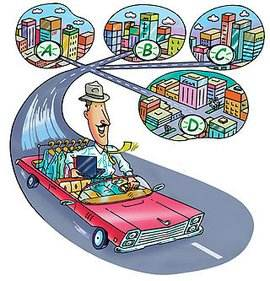
\includegraphics[width=3cm]{pic/bee6.jpg}
		\caption{TSP问题}
	\end{figure}
	\end{columns}
\end{frame}

\begin{frame}
	\frametitle{TSP问题}
	\section {ABC算法应用}
	\begin{columns}
	\column{.6\textwidth}
	\qquad 所有城市的任一种排列即是问题的一个解,因此初始解空间就是N个城市的排列组合。在人工蜂群算法中,将城市个数N作为解空间的维度,每一个蜜源的位置表示其中一个路径的组合,用这条路径的距离长度表示蜜源的适应度,也就是说,适应度越小的蜜源,所表示的路径也就最优。\\
	\qquad 引领蜂和跟随蜂在更新蜜源位置时,是选择其对应的路径中任意两处进行调换生成新的路径,表示新的位置。
	\column{.4\textwidth}
	\begin{table}[]
	\centering
	\caption{TSP与ABC算法映射}
	\label{my-label}
	\begin{tabular}{|l|l|lll}
	\cline{1-2}
	TSP问题     & ABC算法  &  &  &  \\ \cline{1-2}
	访问所有城市的路径 & 蜜源位置   &  &  &  \\ \cline{1-2}
	路径长度      & 蜜源的适应度 &  &  &  \\ \cline{1-2}	
	最短路径      & 最优蜜源   &  &  &  \\ \cline{1-2}
	\end{tabular}
	\end{table}
	\end{columns}
\end{frame}

\begin{frame}
	\frametitle{算法框架}
	\begin{algorithm}[H]
	\caption{ABC on  TSP}\label{bee_alg}
	\algsetup{linenosize=\tiny} \scriptsize
		\begin{algorithmic}
			\STATE{Initialize the parameter: colony size N, maximum number of iteration MaxCycle, limit.}
			\STATE{Initialize the food sources $x_i(i=1,2,3,...,N)$ and compute the fit value.}
			
			\FOR {cycle from 1 to MaxCycle do}
				\FOR {each employee bee i do}
					\STATE {produce a food source $v_{i}$ in the neighbourhood of $X_{i}$; }
					\STATE {Apply greedy selection between of $x_{i}$ and $v_{i}$;}
				\ENDFOR
				\FOR {each onlooker bee i do}
					\STATE {select a food source $x_{i}$ depending on probability pi ; }
					\STATE {produce a food source $v_{i}$ in the neighbourhood of $X_{i}$; }
					\STATE {Apply greedy selection between of $x_{i}$ and $v_{i}$;}
				\ENDFOR
				\IF {there exits an abondoned food source}
					\STATE {Scout bee determines a new food source. }
				\ENDIF
				\STATE {Update best food source;}
			\ENDFOR
		\end{algorithmic}
	\end{algorithm}
\end{frame}

\begin{frame}
	\frametitle{仿真实验}
	\begin{figure}[htbp]
	\begin{minipage}[t]{4cm}
	\centering  
	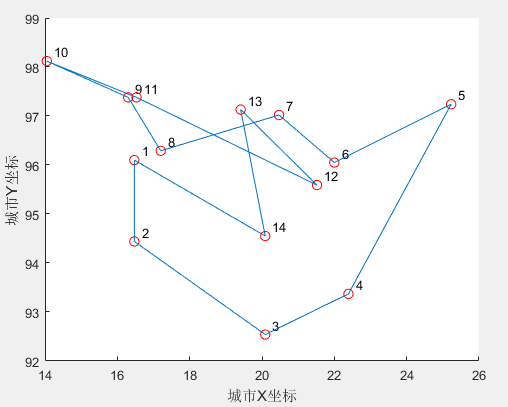
\includegraphics[width=4cm]{pic/bee7.png}  
	\caption{初始路径图}
	\end{minipage}  
	\begin{minipage}[t]{4cm}
	\centering  
	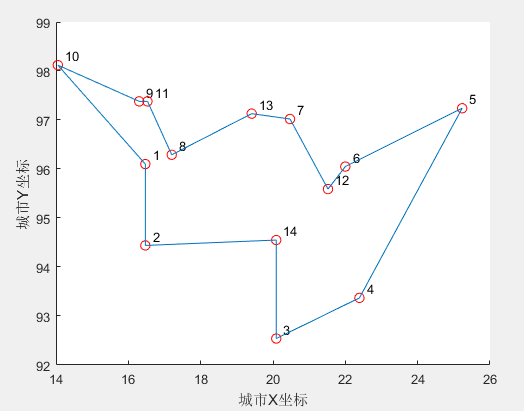
\includegraphics[width=4cm]{pic/bee8.png}  
	\caption{结果路径图}
	\end{minipage}  
	\begin{minipage}[t]{4cm}  
	\flushright
	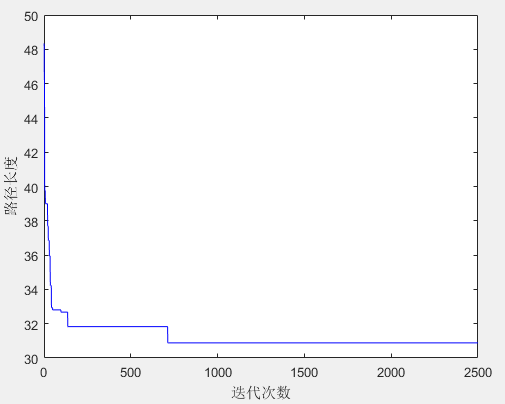
\includegraphics[width=4cm]{pic/bee9.png}  
	\caption{优化曲线}  
	\end{minipage}  
	\end{figure}  
\end{frame}


\begin{frame}
	\frametitle{参考文献}
	\begin{thebibliography}{123456} 
	\bibitem{fish_bib1} 何尧,刘建华,杨荣华.人工蜂群算法研究综述[J/OL].计算机应用研究,2018(05):1-8
	\bibitem{fish_bib2} 陈阿慧,李艳娟,郭继峰.人工蜂群算法综述[J].智能计算机与应用,2014,4(06):20-24
	\bibitem{fish_bib3} Karaboga D. An idea based on honey bee swarm for numerical optimization[R]. Technical report-tr06, Erciyes university, engineering faculty, computer engineering department, 2005.
	\bibitem{fish_bib4} 黄秋菀,王志刚,夏慧明.求解旅行商问题的人工蜂群算法[J].价值工程,2013,32(09):206-207.
	\bibitem{fish_bib5} 魏超.应用人工蜂群算法求解旅行商问题[J].科技视界,2014(19):142-143.
	\end{thebibliography}
\end{frame}


\section{狼群算法}
\begin{frame}
\newcommand{\song}{\setCJKfamilyfont{song}}
\newcommand{\xiaoer}{\fontsize{18pt}{18pt}\selectfont}
	\begin{center}
	{\song\xiaoer\textbf{狼群算法}}
	\end{center}
\end{frame}

\begin{frame}
	\frametitle{GWO背景}
	灰狼优化算法(Grey Wolf Optimizer, GWO)是一种模拟灰狼捕食行为的群体智能算法,该算法最先
	由澳大利亚学者 Mirjalili 于 2014 年提出[1],根据灰狼的社会等级将包围、追捕、攻击等捕食任务分配给不
	同等级的灰狼群来完成捕食行为,从而实现全局优化的过程。 GWO 算法具有操作简单、调节参数少、编
	程易实现等特点。在函数优化方面,与其他群智能优化算法相比有明显的优越性。但同时也存在着易陷
	入局部最优、求解精度不高、收敛速度慢等缺点。
\end{frame}


\begin{frame}
	\frametitle{GWO背景}
	\begin{columns}
	\column{.6\textwidth}
		\begin{itemize}
			\item {狼群中的4个等级}
				\begin{itemize}
					\item {$\alpha$: 头狼,狼群的指挥}
					\item {$\beta$: 辅助头狼进行决策}
					\item {$\delta$: 有经验的老狼,警戒/救助}
					\item {$\omega$: 平衡种群内部关系,协助捕猎}
				\end{itemize}
			\item {狼群的3类行为}
				\begin{itemize}
					\item {跟踪, 追逐, 接近猎物}
					\item {追逐, 包围, 骚扰猎物, 直到猎物停止移动}
					\item {向猎物发起攻击}
				\end{itemize}
		\end{itemize}
	\column{.4\textwidth}
		\begin{figure}[htbp]
			\centering
			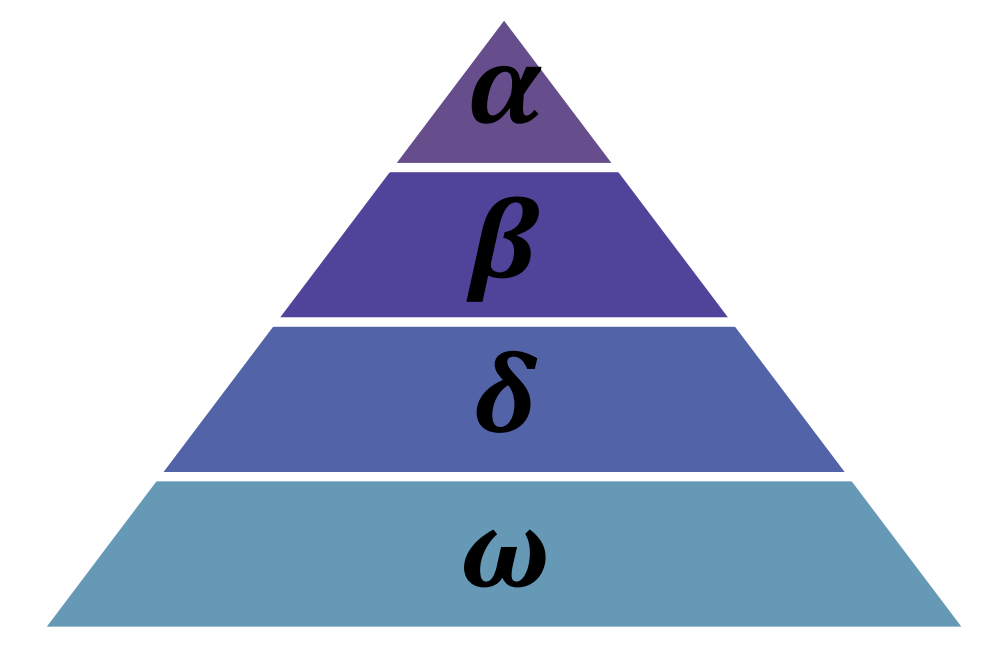
\includegraphics[width=6cm]{pic/wolf1.png}
			\caption{狼群等级结构}
		\end{figure}
	\end{columns}
\end{frame}


\begin{frame}
	\frametitle{GWO背景}
		\begin{figure}[htbp]
			\centering
			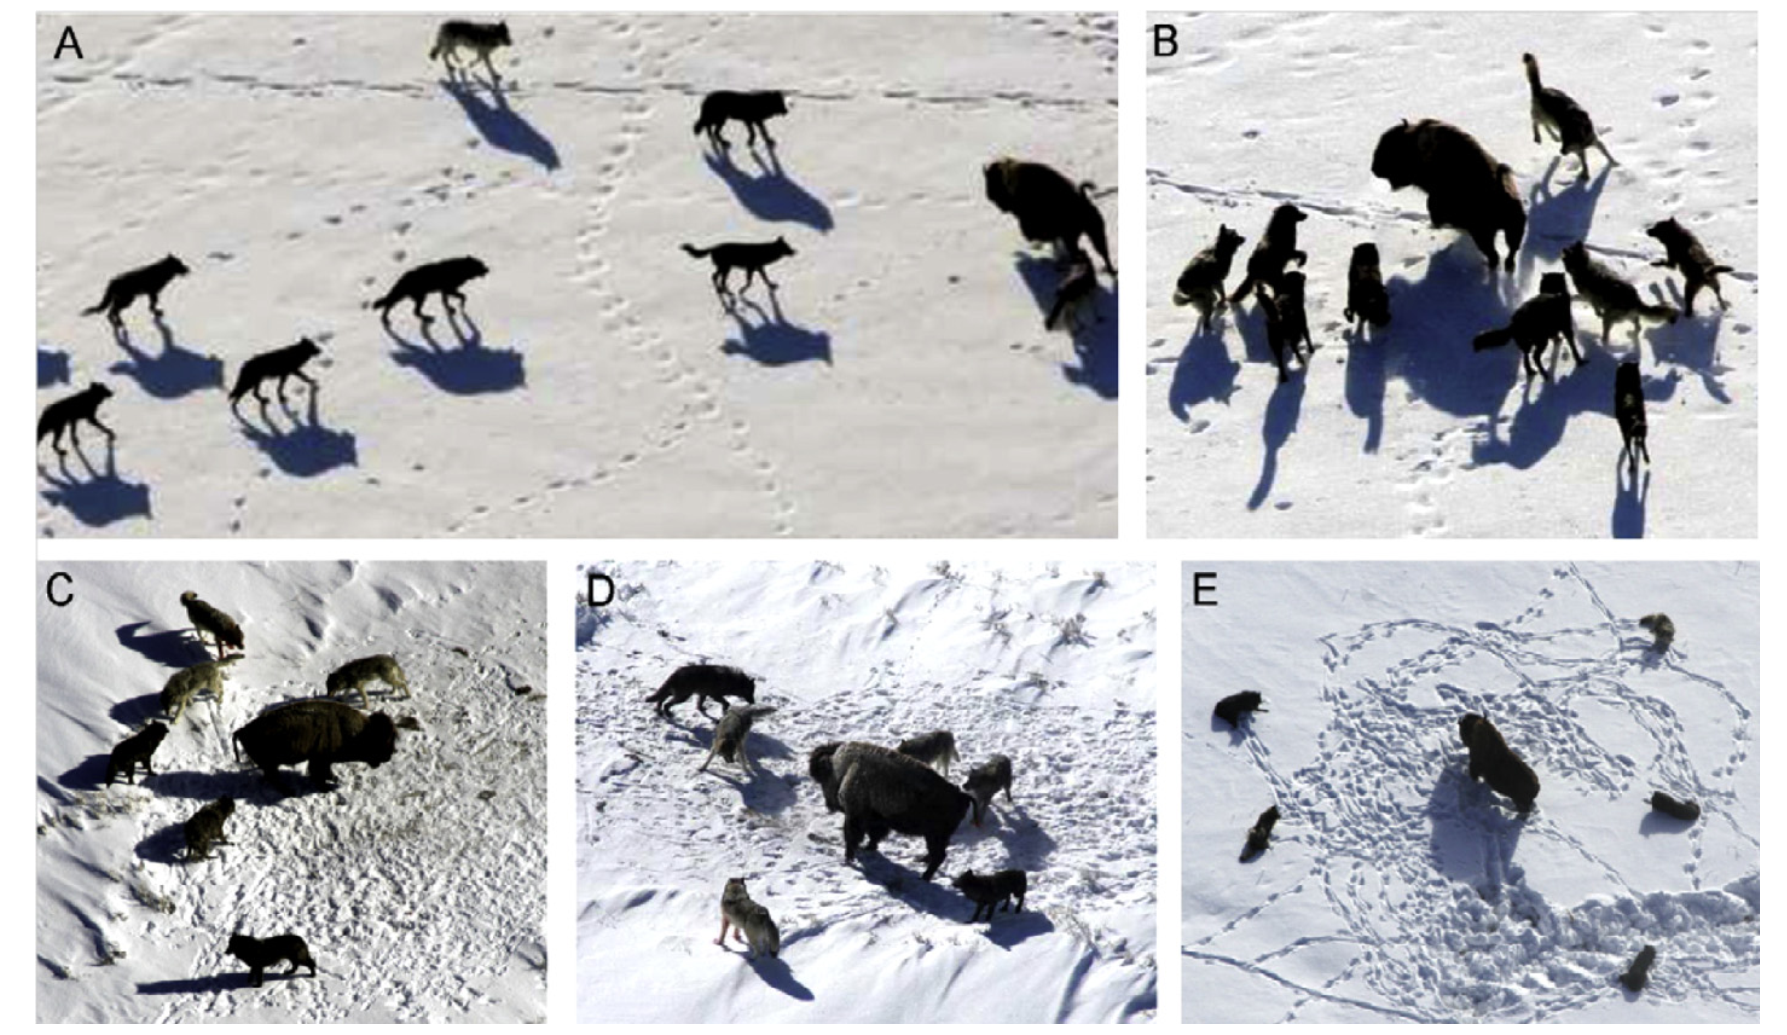
\includegraphics[width=10cm]{pic/wolf2.png}
			\caption{狼群的狩猎行为:A:跟踪猎物;B-D:追逐包围猎物;E:发起攻击}
		\end{figure}
\end{frame}


\begin{frame}
	\frametitle{数学模型——包围/encircling}
	\begin{columns}
	\column{.5\textwidth}
		\begin{equation}
			\vec{D}=|\vec{C} \cdot \vec{X}_{p}(t)-\vec{X}(t)|
		\end{equation}
		\begin{equation}
		\vec{X}(t+1)=\vec{X}(t)-\vec{A}-\vec{D}
		\end{equation}
		其中,$t$代表当前的迭代次数,$\vec{A}$和$\vec{C}$是系数向量,$\vec{X}_p$是当前估计的猎物位置向量,$\vec{X}$是灰狼的位置向量。
		\begin{equation}
			\vec{A}=2\vec{a} \cdot \vec{r}_{1}-\vec{a}
		\end{equation}
		\begin{equation}
		\vec{C}=2 \cdot \vec{r}_2
		\end{equation}
		其中,$\vec{a}$取值在0和2之间,且在迭代过程中逐渐变小,$\vec{r}_1$和$\vec{r}_2$是取值在$[0,1]$之间的随机向量。
	\column{.5\textwidth}
		\begin{figure}[htbp]
			\centering
			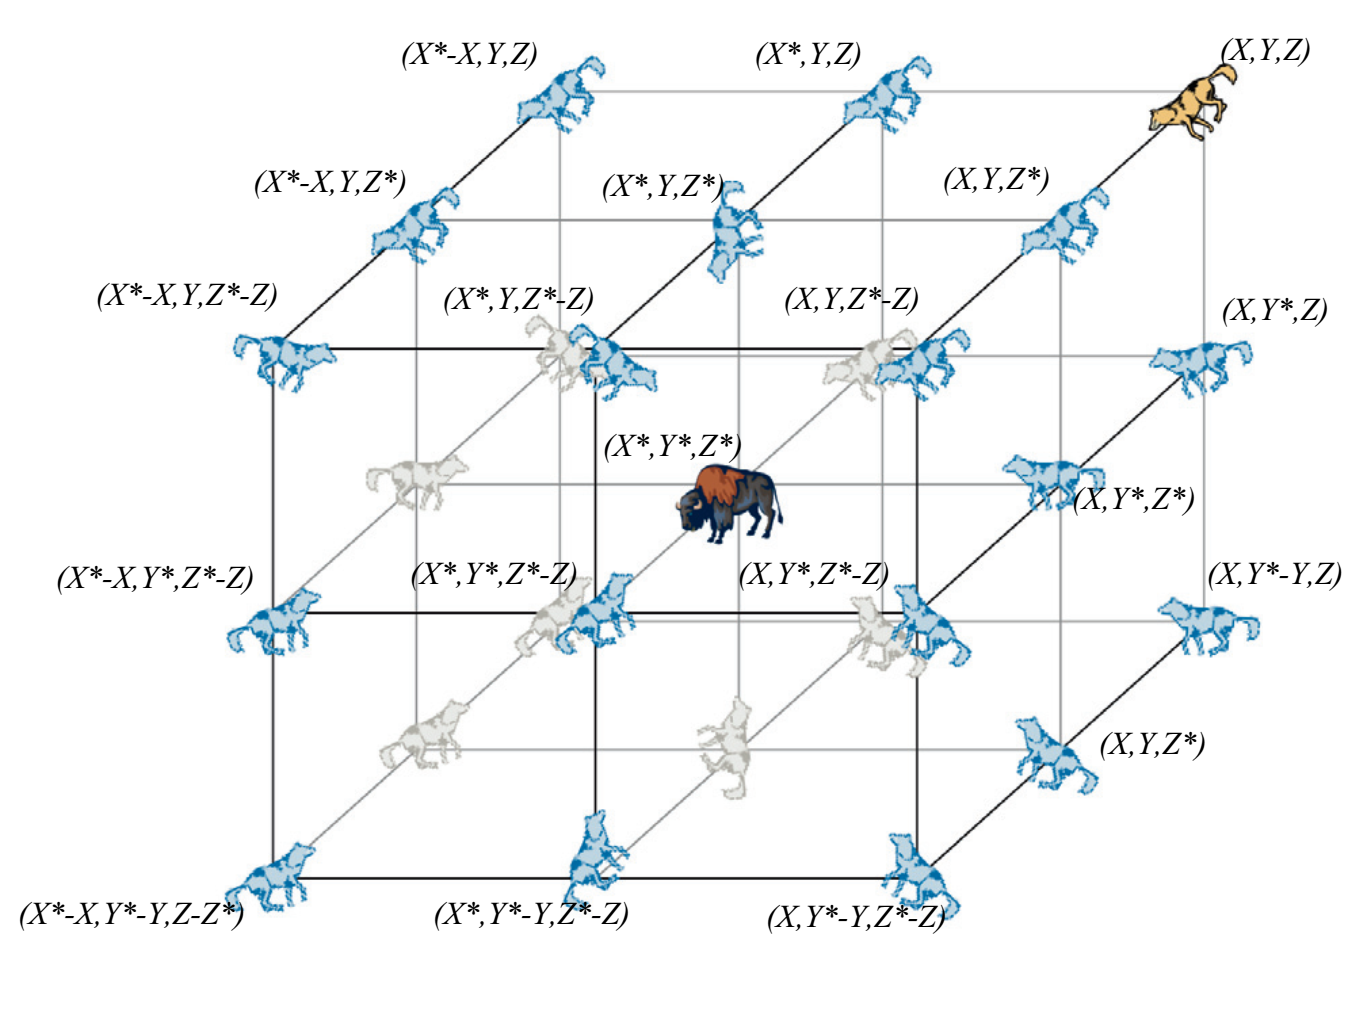
\includegraphics[width=7cm]{pic/wolf3.png}
			\caption{3D空间中灰狼的下一个可能位置}
		\end{figure}
	\end{columns}
\end{frame}


\begin{frame}
	\frametitle{数学模型——捕猎/hunting}
	\begin{itemize}
		\item {实际上,猎物位置$\vec{X}_p$是未知的}
		\item {假设把$\alpha$狼的位置作为最佳候选解,$\beta$和$\delta$次之}
		\item {根据这三个较优解,狼群的每个个体开始进行移动}
	\end{itemize}
	\begin{align}
	&\vec{D}_{\alpha}=|\vec{C}_1 \cdot \vec{X}_{\alpha}-\vec{X}|,\quad \vec{D}_{\beta}=|\vec{C}_2 \cdot \vec{X}_{\beta}-\vec{X}|,\quad \vec{D}_{\delta}=|\vec{C}_3 \cdot \vec{X}_{\delta}-\vec{X}| \\
	&\vec{X}_1=\vec{X}_{\alpha}-\vec{A}_1 \cdot \vec{D}_{\alpha},\quad \vec{X}_2=\vec{X}_{\beta}-\vec{A}_2 \cdot \vec{D}_{\beta},\quad \vec{X}_3=\vec{X}_{\delta}-\vec{A}_3 \cdot \vec{D}_{\delta} \\
	&\vec{X}(t+1)=\cfrac{\vec{X}_1+\vec{X}_2+\vec{X}_3}{3}
	\end{align}
\end{frame}

\begin{frame}
	\frametitle{数学模型——捕猎/hunting}
	\begin{figure}[htbp]
		\centering
		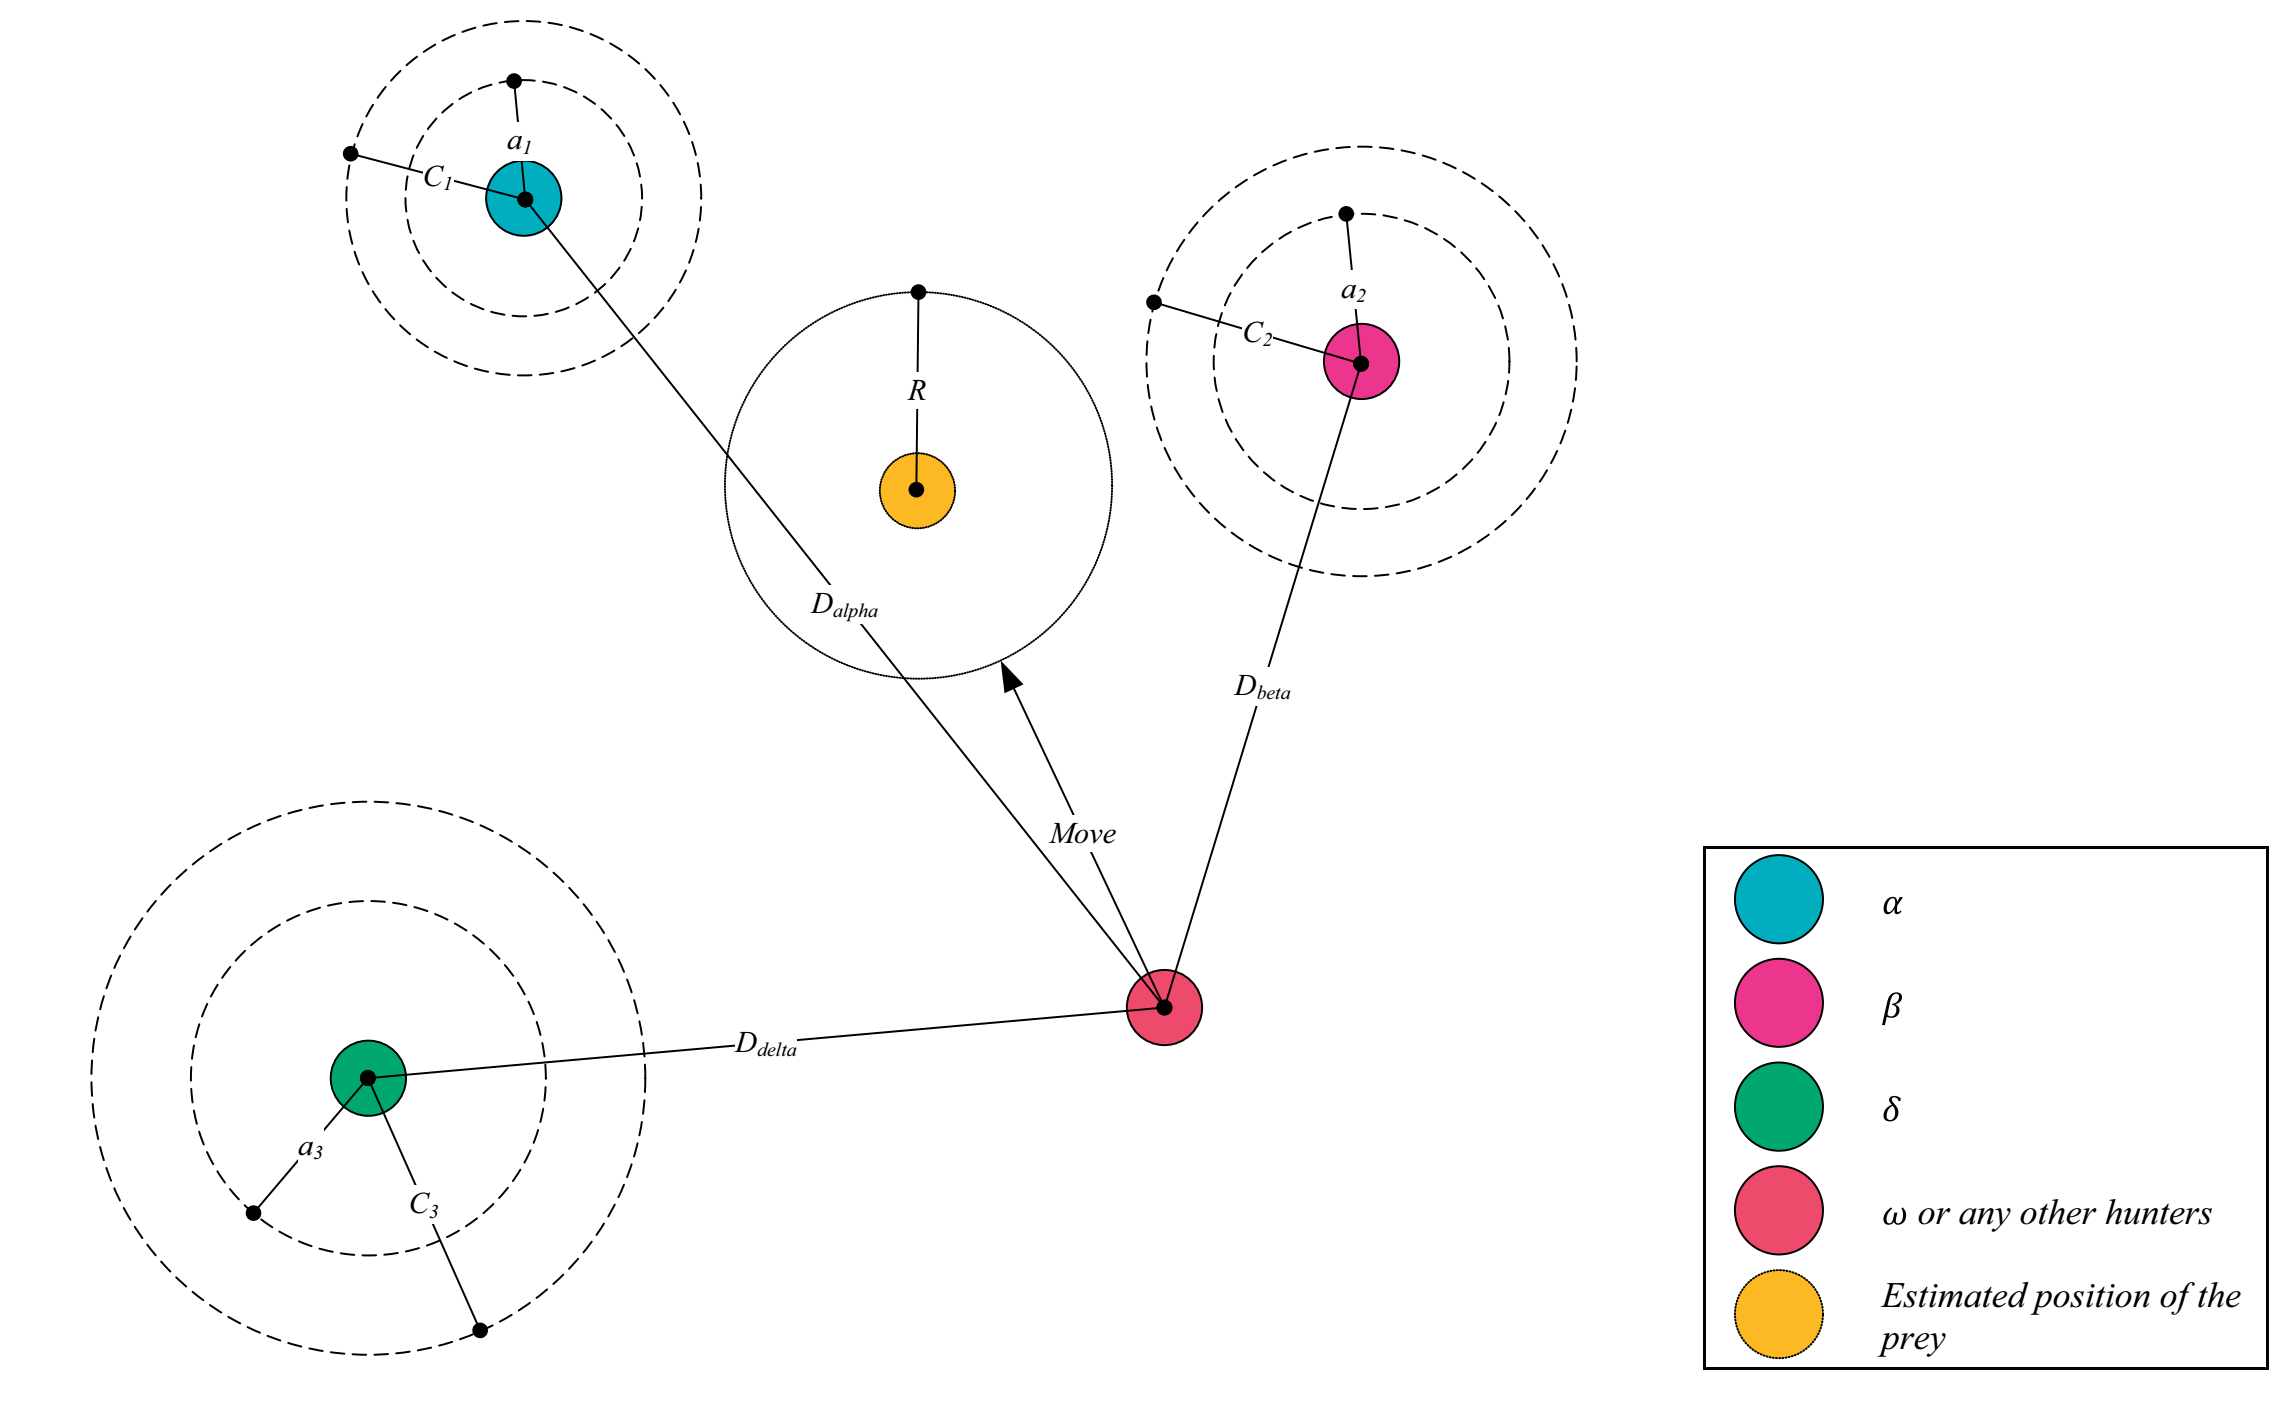
\includegraphics[width=10cm]{pic/wolf4.png}
		\caption{狼群hunting行为示意图}
	\end{figure}
\end{frame}

\begin{frame}
	\frametitle{数学模型——攻击搜寻/attacking,exploration}
	\begin{columns}
	\column{.4\textwidth}
		\begin{itemize}
			\item {Attacking prey (exploitation)}
				\begin{itemize}
					\item {当猎物停止移动时,狼群会发起攻击}
					\item {该过程由a的递减实现,A在[-a,+a]之间变化}
					\item {当|A|<1时,狼群的下一个位置会更加接近猎物位置}
				\end{itemize}
			\item {Search for prey (exploration)}
				\begin{itemize}
					\item {当$|A|>1$时,狼群会远离猎物位置}
					\item {$C$可以看做狼群接近猎物的障碍,它影响了狼和猎物之间距离的衡量,这种游走行为会降低陷入局部最优解的可能性}
				\end{itemize}
		\end{itemize}
	\column{.6\textwidth}
		\begin{figure}[htbp]
			\centering
			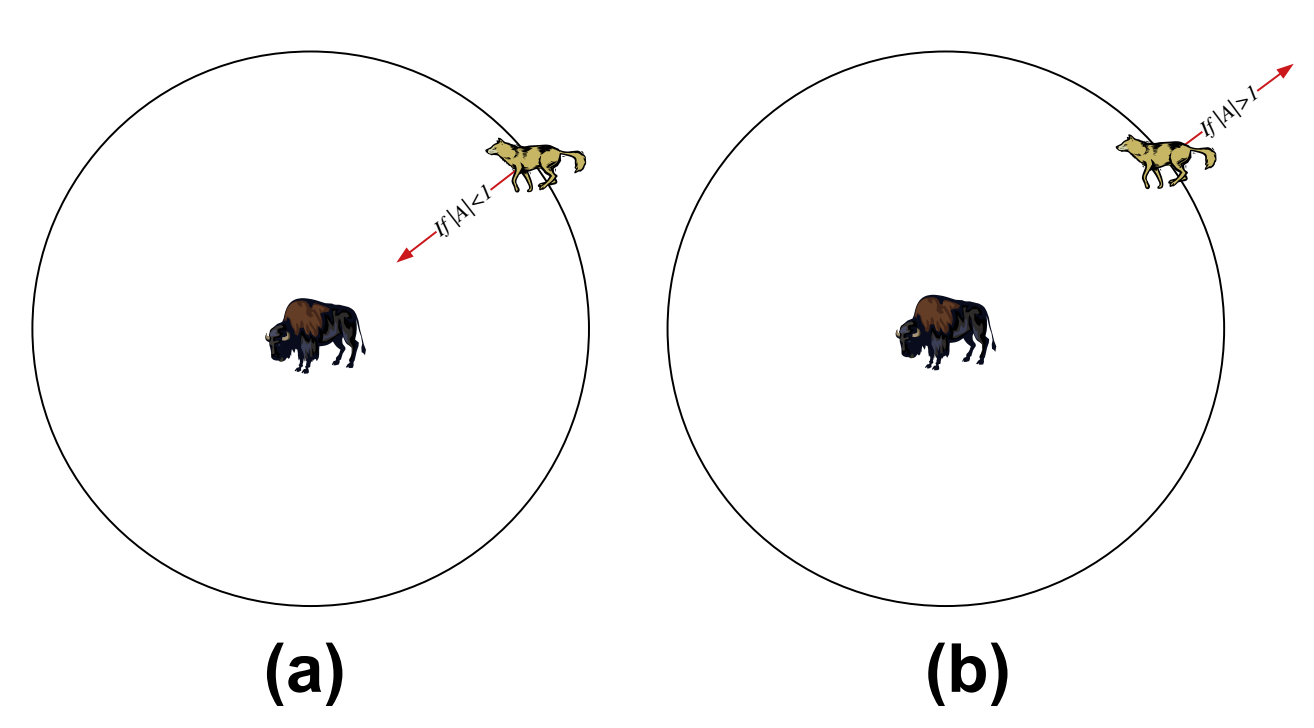
\includegraphics[width=7cm]{pic/wolf5.png}
			\caption{攻击猎物(a)和搜寻猎物(b)}
		\end{figure}
	\end{columns}
\end{frame}


\begin{frame}
	\frametitle{GWO算法}
	\begin{algorithm}[H]
	\caption{GWO}\label{wolf_alg}
	\algsetup{linenosize=\tiny} \scriptsize
		\begin{algorithmic}
			\STATE{Initialize the grey wolf population $X_i(i=1,2,3,...,n)$}
			\STATE{Initialize a, A and C}
			\STATE{Calculate the fitness of each search agent}
			\STATE{$X_{\alpha}$: the best search agent}
			\STATE{$X_{\beta}$: the second best search agent}
			\STATE{$X_{\delta}$: the third best search agent}
			\WHILE{$t < $ Max number of iterations}
				\FOR{each search agent}
					\STATE{Update the position of current search agent}
				\ENDFOR
				\STATE{Update a, A and C}
				\STATE{Caulate the fitness of all aearch agents}
				\STATE{Update $X_{\alpha}$, $X_{\beta}$ and $X_{\delta}$}
				\STATE{$t=t+1$}
			\ENDWHILE
			\STATE{return $X_{\alpha}$}
		\end{algorithmic}
	\end{algorithm}
\end{frame}

\begin{frame}
	\frametitle{Benchmark-unimodal}
	\begin{table}[]
	\centering
	\caption{unimodal functions}
	\label{wolf_table1}
	\begin{tabular}{lccc}
	\hline
	function & dim & range & $f_{min}$ \\ \hline \hline
	$f_1(x)=\sum_{i=1}^{n}x_i^2$ & 30 &  [-100,100]  & 0  \\ \hline
	$f_2(x)=\sum_{i=1}^{n}|x_i|+\prod_{i=1}^{n}|x_i|$ & 30 & [-10,10] & 0 \\ \hline
	$f_3(x)=\sum_{i=1}^{n}(\sum_{j-1}^{i} x_j)^2$ & 30  & [-100,100] &  0 \\ \hline
	$f_4(x)=max_i\{|x_i|,1 \leq i\leq n\}$ & 30 & [-100,100] &  0 \\ \hline
	$f_5(x)=\sum_{i=1}^{n-1}[100(x_{i+1}-x_i^2)^2+(x_i-1)^2]$ & 30 & [-30,30] &  0 \\ \hline
	\end{tabular}
	\end{table}
\end{frame}


\begin{frame}
	\frametitle{Benchmark-multimodal}
	\begin{table}[]
	\centering
	\caption{multimodal functions}
	\label{wolf_table2}
	\begin{tabular}{p{8cm}lccc}  
	\hline
	function & dim & range & $f_{min}$ \\ \hline \hline
	$f_6(x)=\sum_{i=1}^{n} -x_i \sin (\sqrt{|x_i|})$ & 30 &  [-500,500]  & $-418.9829 \times 5$ \\ \hline
	$f_7(x)=\sum_{i=1}^{n}[x_i^2-10\cos (2 \pi x_i)+10]$ & 30 & [-5.12,5.12] & 0 \\ \hline
	$f_8(x)=-20\exp{\left(-0.2\sqrt{\frac{1}{2}\sum_{i=1}^{n}x_i^2}\right)}- \exp{\left(\frac{1}{n}\sum_{i=1}^{n}\cos(2\pi x_i)\right)+20+e}$ & 30  & [-32,32] &  0 \\ \hline
	$f_9(x)=\frac{1}{4000}\sum_{i=1}{n}x_1^2-\prod_{i=1}^{n}\cos\left(\frac{x_1}{\sqrt{i}} \right)+1 $ & 30 & [-600,600] &  0 \\ \hline
	$f_{10}(x)=\frac{\pi}{n}\{10\sin(\pi y_i)+\sum_{i=1}^{n-1}(y_i-1)^2  [1+10{\sin}^2(\pi y_{i+1})]+(y_n-1)^2\}+\sum_{i=1}^{n}u(x_i,10,100,4) $ & 30 & [-50,50] &  0 \\ \hline
	\end{tabular}
	\end{table}
\end{frame}

\begin{frame}
	\frametitle{Something about PSO}
		\begin{figure}[htbp]
			\centering
			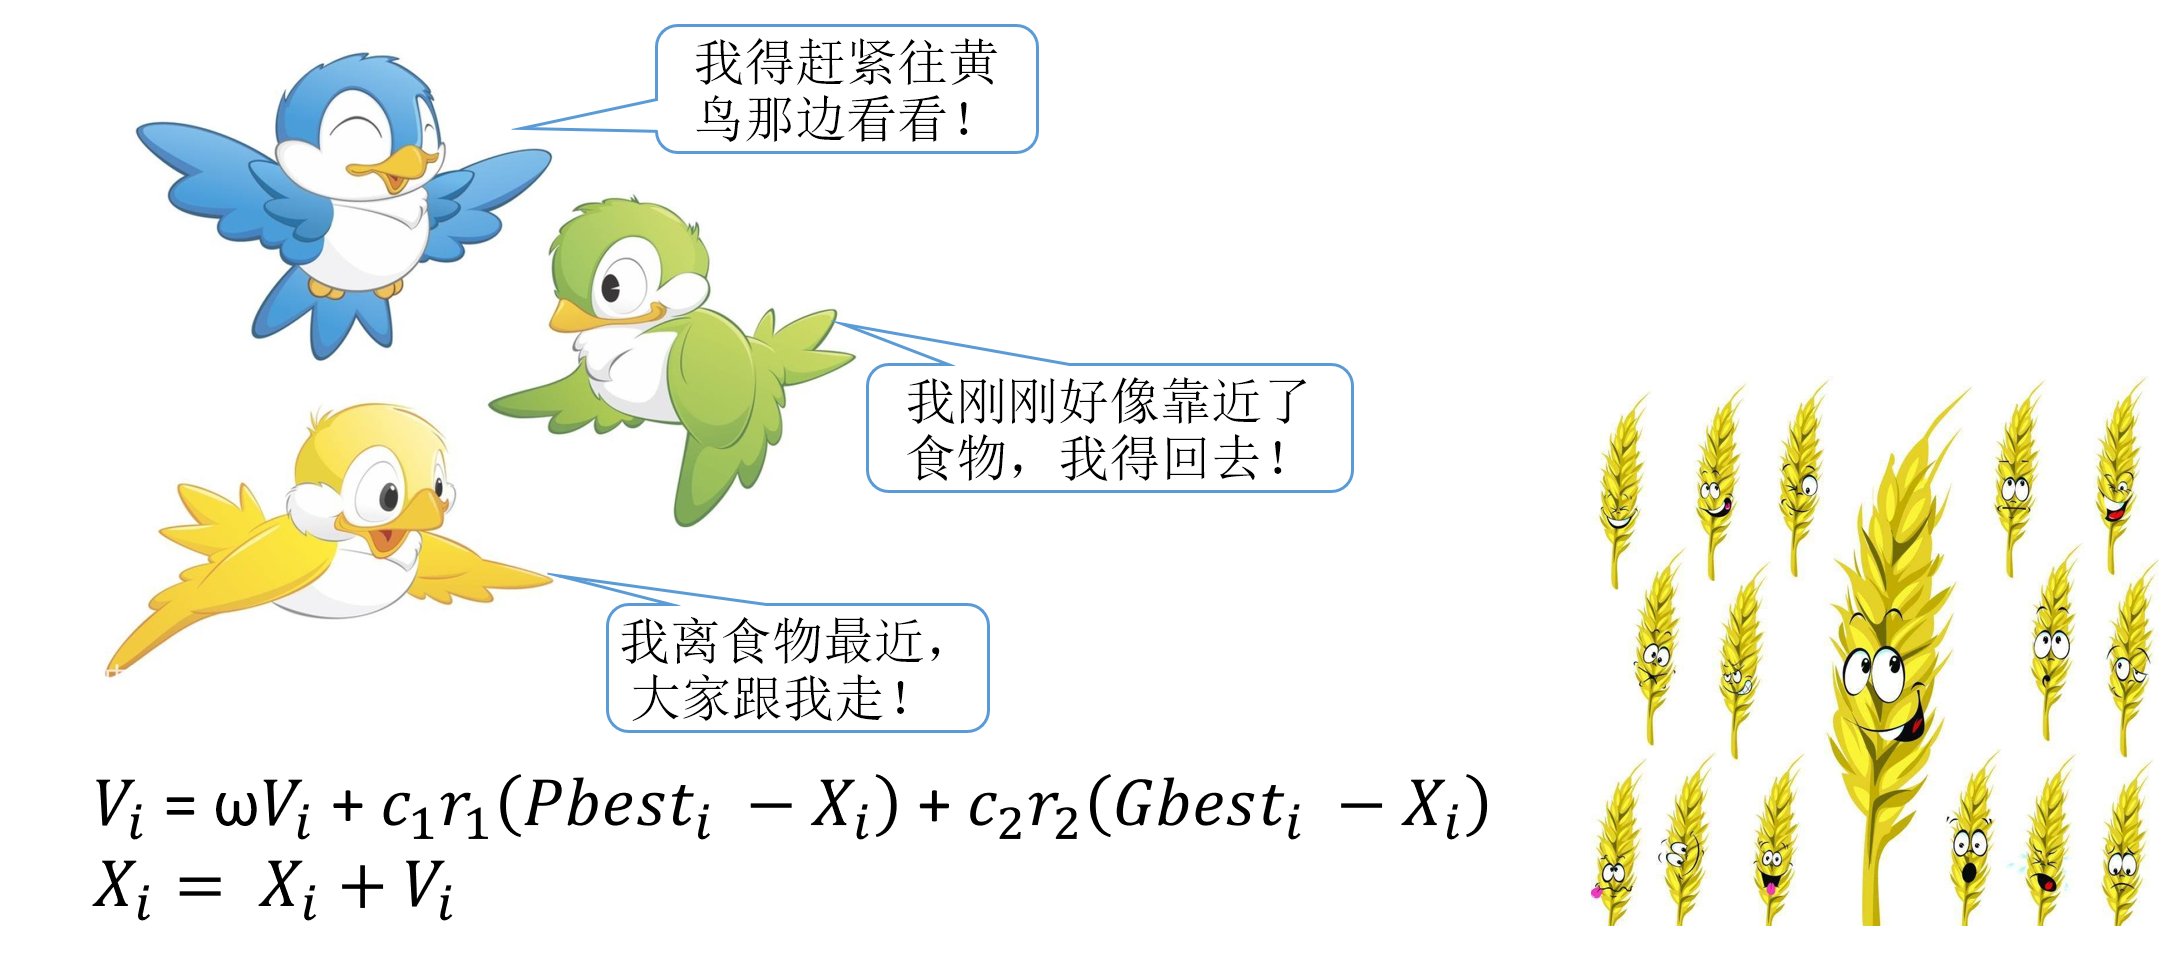
\includegraphics[width=14cm]{pic/wolf6.png}
		\end{figure}
\end{frame}

\begin{frame}
	\frametitle{实验结果}
	\begin{table}[]
	\centering
	\caption{GWO与PSO对比}
	\label{wolf_table3}
	\begin{tabular}{cccccc}
	\multirow{2}{*}{function} & \multirow{2}{*}{min} & \multicolumn{2}{c}{GWO} & \multicolumn{2}{c}{PSO} \\ \cline{3-6} 
	                          &                      & ave        & std        & ave        & std        \\ \hline
	F1                        & 0                    & 6.59e-28   & 6.34e-05   & 1.36e-04   & 2.02e-04   \\
	F2                        & 0                    & 7.18e-17   & 0.029      & 4.21e-02   & 0.045      \\
	F3                        & 0                    & 3.29e-06   & 79.149     & 70.125     & 22.119     \\
	F4                        & 0                    & 5.61e-07   & 1.315      & 1.086      & 0.317      \\
	F5                        & 0                    & 26.81258   & 69.904     & 96.718     & 60.116     \\
	F6                        & -2094.91             & -6123.1    & -4087.44   & -4841.3    & 1152.814   \\
	F7                        & 0                    & 0.310      & 47.356     & 46.704     & 11.629     \\
	F8                        & 0                    & 1.06e-13   & 0.078      & 0.276      & 0.509      \\
	F9                        & 0                    & 0.004      & 0.007      & 0.009      & 0.008      \\
	F10                       & 0                    & 0.053      & 0.020      & 0.007      & 0.026     
	\end{tabular}
	\end{table}
\end{frame}


\begin{frame}
	\frametitle{GWO改进}
	GWO 算法具有操作简单、调节参数少、编程易实现等特点。在函数优化方面,与其他群智能优化算法相比有明显的优越性。但同时也存在着易陷入局部最优、求解精度不高、收敛速度慢等缺点。
	\begin{itemize}
		\item {采用计算分配值的方法提出一种自适应搜索的灰狼求解算法从而加快算法的收敛速度[2]}
		\item {将混沌序列方法引入初始化种群个体,给出了一种寻优性和鲁棒性更好的改进 GWO 算法[3]}
		\item {引入了佳点集理来初始化狼群,并用非固定多段映射罚函数法处理约束条件,利用改进 GWO 算法求解约束优化问题[4]}
	\end{itemize}
	小生境灰狼优化算法(Niche Grey Wolf Optimization, NGWO)[5]利用基本 GWO 算法计算每个灰狼的适应度值。当灰狼距离小于生存半径时,对适应度较差的个体施加惩罚函数,以提高全局搜索能力。
\end{frame}


\begin{frame}
	\frametitle{小生境灰狼算法NGWO}
	\begin{columns}
	\column{.5\textwidth}	
	\begin{itemize}
		\item {“人以类聚,物以群分”}
		\item {将种群划分为多个小生境种群,一小群体为单位进化}
		\item {对小生境种群中适应度较差的个体施加惩罚}
	\end{itemize}
	\column{.5\textwidth}
	个体间距离采用欧氏距离:
	$$d_{ij}=||X_i-X_j||$$
	小生境群体:
	$$d_{ij} < \sigma_{share}$$
	\end{columns}	
\end{frame}


\begin{frame}
	\frametitle{NGWO算法}
	\begin{algorithm}[H]
	\caption{NGWO}\label{nwolf_alg}
	\algsetup{linenosize=\tiny} \scriptsize
		\begin{algorithmic}
			\STATE{Initialize the grey wolf population $X_i(i=1,2,3,...,n)$}
			\STATE{Initialize a, A, C and penatly}
			\STATE{Calculate the fitness $f_i$ of each search agent}
			\STATE{$X_{\alpha}$: the best search agent}
			\STATE{$X_{\beta}$: the second best search agent}
			\STATE{$X_{\delta}$: the third best search agent}
			\WHILE{$t < $ Max number of iterations}
				\FOR{each search agent}
					\STATE{Update the position of current search agent}
				\ENDFOR
				\STATE{Caculate the distance matrix}
				\IF{$d_{ij}<\sigma{share}$}
					\STATE{Set $min\left(f_i,f_j \right)=penalty$}
				\ENDIF
				\STATE{Update a, A and C}
				\STATE{Caulate the fitness of all aearch agents}
				\STATE{Update $X_{\alpha}$, $X_{\beta}$ and $X_{\delta}$}
				\STATE{$t=t+1$}
			\ENDWHILE
			\STATE{return $X_{\alpha}$}
		\end{algorithmic}
	\end{algorithm}
\end{frame}


\begin{frame}
	\frametitle{参考文献}
	\begin{thebibliography}{99} 
	\bibitem{wolf_bib1} Mirjalili, S., Mirjalili, S. and Lewis, A. (2014) Grey Wolf Optimizer. \emph{Advances in Engineering Software}, 69, 46-61
	\bibitem{wolf_bib2} 罗佳, 唐斌. 新型灰狼优化算法在函数优化中的应用[J]. 兰州理工大学学报, 2016, 6(3): 97-101  
	\bibitem{wolf_bib3} 魏政磊, 赵辉, 韩邦杰, 等. 基于自适应 GWO 的多 UCAV 协同攻击目标决策[J]. 计算机工程与应用, 2016, 25(18): 97-101
	\bibitem{wolf_bib4} 龙文, 赵东泉, 等. 求解约束优化问题的改进灰狼优化算法[J]. 计算机应用, 2015, 35(9): 2590-2595
	\bibitem{wolf_bib5} 白媛, 陈京荣, 展之婵. 改进灰狼优化算法的研究与分析[J]. 计算机科学与应用, 2017, 7(6): 562-571
	\end{thebibliography}
\end{frame}

\section{猫群算法}
\begin{frame}
  \frametitle{cat}
	 \begin{enumerate}
	    \item test
	    \item test
	    \item test
	    \item test
	  \end{enumerate}
\end{frame}

\section{鲸群算法}
%example

\begin{frame}
  \frametitle{鲸鱼优化算法}

	 \begin{enumerate}
	    \item 面向问题
	    \item 灵感来源
	    \item 模型建立
	    \item 算法步骤
	    \item 评价
	  \end{enumerate}
\begin{picture}(1,1)
\put(75,0){
\includegraphics[width=0.6\textwidth]{pic/whale_author.png}}
\end{picture}
\end{frame}


\begin{frame}
  \frametitle{要解决什么优化问题?}
	\begin{itemize}
	\item {形如各种基准函数的优化问题}
	\end{itemize}
\begin{figure}
\centering
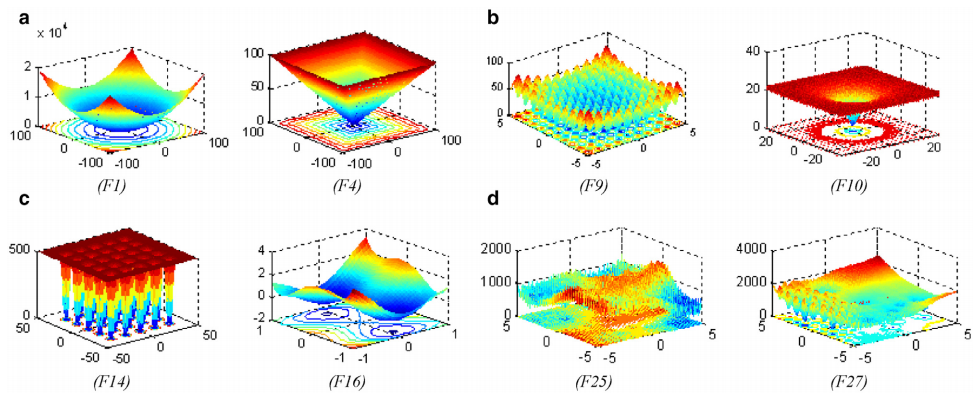
\includegraphics[width=1\textwidth]{pic/whale_function.png}
\end{figure}
\end{frame}

\begin{frame}
  \frametitle{要解决什么优化问题?}
	\begin{itemize}
	\item {实际工程中带有不同约束的优化问题}
	\end{itemize}
\begin{figure}
\centering
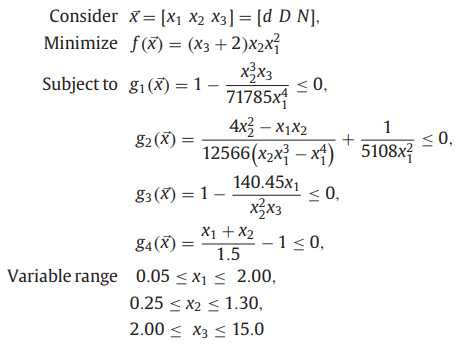
\includegraphics[width=0.6\textwidth]{pic/whale_constraint.png}
\end{figure}
\end{frame}

\begin{frame}
  \frametitle{灵感来源---驼背鲸的捕食行为}
	\begin{block}{制造圆形或螺旋结构的气泡网,收缩包围猎物。}
	\url{http://tv.cntv.cn/video/C36795/3912f2138bca4b15a39c21b17f85116c}
	 \end{block}
\begin{figure}
\centering
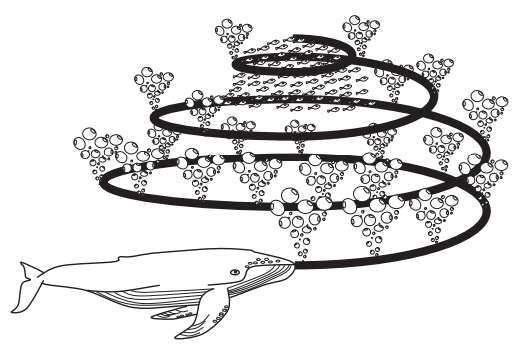
\includegraphics[width=0.6\textwidth]{pic/whale_humpback.png}
\end{figure}

\end{frame}

\begin{frame}
  \frametitle{模型建立}
	\begin{itemize}
	\item {鲸鱼群:在搜索空间中的要搜索的位置}
	\item {猎物:最优解所在位置}
	\end{itemize}
	\begin{block} {\qquad 即在搜索空间中用一群鲸鱼,围绕着当前搜索到的猎物(局部最优解)不断移动位置(迭代更新搜索位置),去寻找猎物更多的位置(最优解)。}
	    \vspace{3mm}
	     \begin{itemize}
	\item {开发阶段(位置更新策略):圆形收缩、螺旋收缩}
	\item {探索阶段(避免局部最优):从比当前位置离局部最优解更远的位置向局部最优解收缩包围}
	\end{itemize}
	\end{block}
	
\end{frame}

\begin{frame}
	\frametitle{模型建立---开发阶段(圆形收缩)}
	\begin{block}{
		\begin{displaymath} \vec{D}= \left | \vec{C}\cdot\vec{X^{*}}(t)-\vec{X}(t) \right | \eqno(1)  \end{displaymath}
		\begin{displaymath} \vec{X}(t+1)=\vec{X^{*}}(t)-\vec{A}\cdot \vec{D} \eqno(2)  \end{displaymath}
	}
	\begin{itemize}
		\item $t$当前迭代    \qquad $\vec{A},\vec{C}$系数向量
		\item $\vec{X^{*}}$当前局部最优解的位置向量,不断更新局部最优解
		\item $\vec{X}$位置向量
		\item $\left | \right |$绝对值    \qquad$\cdot$对应元素相乘
	\end{itemize}
	\end{block}
	\begin{block}{
	\begin{displaymath} \vec{A}=2\vec{a}\cdot\vec{r}-\vec{a} \eqno(3)\end{displaymath}
	\begin{displaymath} \vec{C}=2\cdot\vec{r} \eqno(4)\end{displaymath}
	}
	\begin{itemize}
		\item $\vec{a}$随着迭代过程,从2到0线性递减的向量
		\item $\vec{r}$随机向量,值在[0,1]之间
	\end{itemize}
	\end{block}

	
\end{frame}

\begin{frame}
  \frametitle{模型建立---开发阶段(圆形收缩)图示}
\begin{figure}
\centering
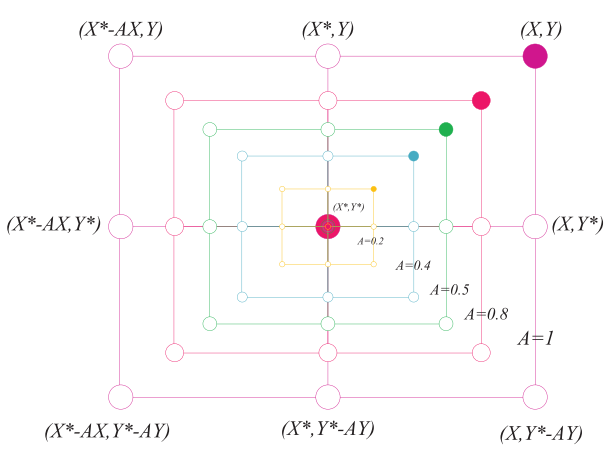
\includegraphics[width=0.6\textwidth]{pic/whale_exploitation1.png}
\end{figure}
\end{frame}

\begin{frame}
  \frametitle{模型建立---开发阶段(螺旋收缩)}
	\begin{block}{
	\begin{displaymath} \vec{X}(t+1)=\vec{{D}'}\cdot e^{bl}\cdot cos(2\pi l)+\vec{X^{*}}(t) \eqno(5)\end{displaymath}}
	\begin{itemize}
		\item $\vec{{D}'}=|\vec{X^{*}}(t)-\vec{X}(t)|$某个鲸鱼离局部最优解的距离(向量的绝对值)
		\item $b$常数,定义对数螺线
		\item $l$随机数,值在[-1,1]
		\item $\cdot$对应元素相乘
	\end{itemize}
	\end{block}
	
\end{frame}

\begin{frame}
  \frametitle{模型建立---开发阶段(螺旋收缩)图示}
\begin{figure}
\centering
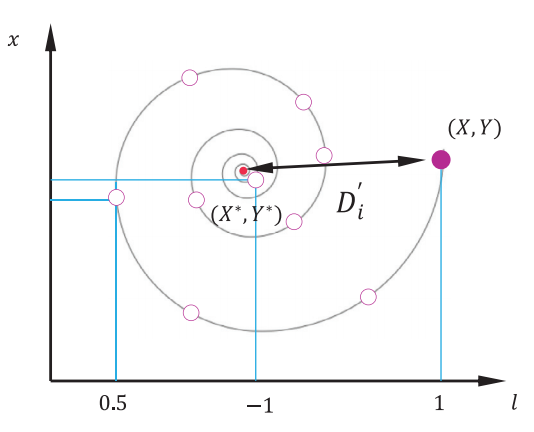
\includegraphics[width=0.6\textwidth]{pic/whale_exploitation2.png}
\end{figure}
\end{frame}

\begin{frame}
  \frametitle{模型建立---开发阶段(两种方式结合)}
	\begin{block}{ 
	\begin{displaymath}
	\vec{X}(t+1)=\begin{cases}
	\vec{X^{*}}(t)-\vec{A}\cdot \vec{D} & \text{ if } p<0.5 \\ 
	\vec{{D}'}\cdot e^{bl}\cdot cos(2\pi l)+\vec{X^{*}}(t) & \text{ if } p\geq 0.5 
	\end{cases}
	\eqno(6)\end{displaymath}
  }
  \begin{itemize}
		\item $p$随机数,值在[0,1]
	\end{itemize}
  \end{block}
 \end{frame}


\begin{frame}
  \frametitle{模型建立---探索阶段(避免局部最优)}
	\begin{block}{
	\begin{displaymath} \vec{D}=|\vec{C}\cdot \vec{X}_{rand}-\vec{X}| \eqno(7)\end{displaymath}
	\begin{displaymath} \vec{X}(t+1)=\vec{X}_{rand}-\vec{A}\cdot \vec{D} \eqno(8)  \end{displaymath}
	}
	\begin{itemize}
		\item $\vec{X}_{rand}$一个随机位置(一条随机的鲸鱼)
	\end{itemize}
	\end{block}
	
\end{frame}

\begin{frame}
  \frametitle{模型建立---探索阶段(避免局部最优)图示}
	\begin{figure}
\centering
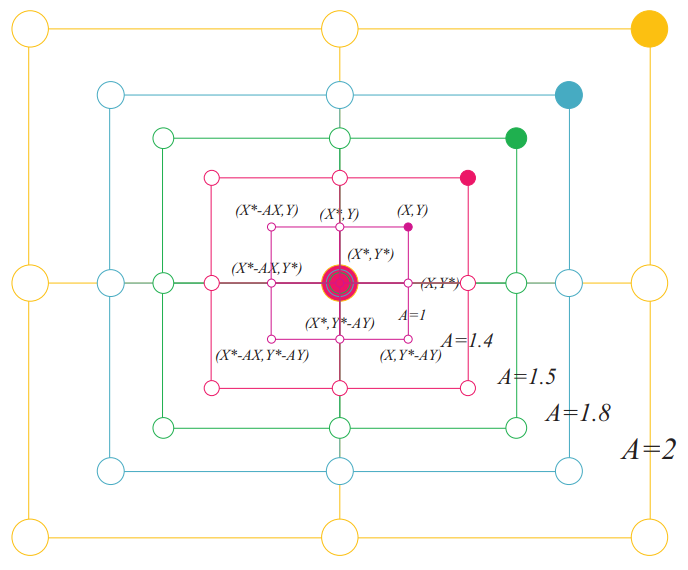
\includegraphics[width=0.6\textwidth]{pic/whale_exploration.png}
\end{figure}
	
\end{frame}



\begin{frame}
  \frametitle{算法步骤}
 Initialize\ the\ whales\ population\ $X_{i}$ (i = 1, 2, ..., n)\\
 Calculate\ the\ fitness\ of\ each\ search\ agent\\
 $X^{*}$=the\ best\ search\ agent\\
 \textbf{\emph{while}} (t < maximum\ number\ of\ iterations)\\
 \qquad \textbf{\emph{for}}\ each\ search\ agent\\
 \qquad Update\ a, A, C, l, and\ p\\
 \qquad \qquad \textbf{\emph{if1}} (p<0.5)\\
 \qquad \qquad \qquad \textbf{\emph{if2}} (|A| < 1)\\
 \qquad \qquad \qquad \qquad Update\ the\ position\ of\ the\ current\ search\ agent\ by\ the\ Eq. (2)\\
 \qquad \qquad \qquad \textbf{\emph{else if2}} ($|A|\geq 1$)\\
 \qquad \qquad \qquad \qquad Select\ a\ random\ search\ agent ($X_{rand}$)\\
 \qquad \qquad \qquad \qquad Update\ the\ position\ of\ the\ current\ search\ agent\ by\ the\ Eq. (8)\\
 \qquad \qquad \qquad \textbf{\emph{end if2}}\\
 \qquad \qquad \textbf{\emph{else if1}} ($p\geq  0.5$)\\
 \qquad \qquad \qquad Update\ the\ position\ of\ the\ current\ search\ by\ the\ Eq. (5)\\
 \qquad \qquad \textbf{\emph{end if1}}\\
 \qquad \textbf{\emph{end for}}\\
\end{frame}

\begin{frame}
  \frametitle{算法步骤}

 \qquad Check\ if\ any\ search\ agent\ goes\ beyond\ the\ search\ space\ and\ amend\ it\\
 \qquad Calculate\ the\ fitness\ of\ each\ search\ agent\\
 \qquad Update\ $X^{*}$\ if\ there\ is\ a\ better\ solution\\
 \qquad $t=t+1$\\
 \textbf{\emph{end while}}\\
 return X*
\end{frame}


\begin{frame}
  \frametitle{评价}
\begin{block}{相较于PSO(粒子群)、GSA(引力搜索)、DE(差分进化)、FEP(快速进化规划)、CMA-ES(协方差矩阵自适应进化)等算法
	}
	\begin{itemize}
		\item 开发能力(单峰函数优化能力)
			\begin{itemize}
				\item 大多测试函数上,排第一到第二位。
			\end{itemize}
		\item 探索能力(多峰函数优化能力)
		\begin{itemize}
				\item 大多测试函数上,排第一到第二位。
			\end{itemize}
		\item 跳出局部最优能力
		\begin{itemize}
				\item 3/7测试函数排第一,3/7个函数问题排第二。
			\end{itemize}
		\item 收敛行为
		\begin{itemize}
				\item 在某些函数上,呈现出较快的后期收敛速度。
			\end{itemize}
	\end{itemize}
	Mirjalili S, Lewis A. The Whale Optimization Algorithm[J]. Advances in Engineering Software, 2016, 95:51-67.
	\end{block}
	
\end{frame}




\section{结论}
\begin{frame}
  \frametitle{结论}

  \begin{itemize}
    \item Easy to use
    \item Good results
  \end{itemize}
\end{frame}


\section{参考文献}
\begin{frame}{参考文献}
\begin{thebibliography}{99} 
\bibitem{zhao1} Yi~Zhao, {\sl An introduction to X}, Sep.~15, 2015
\bibitem{qian2} Er~Qian, San~Sun, 
Phys.\ Lett.\ A {\bf xx}, 2xx (20xx)   
\bibitem{li4} Si~Li, Phys.\ Rev.\ C {\bf xx}, 5xx (20xx) 
\end{thebibliography}
\end{frame}

\end{document}